\documentclass[a4paper]{article}
\def\DOCTITLE{CSC3121 Distributed Systems}
% Set document attributes
\title{\DOCTITLE}

\usepackage{fullpage}
\usepackage{scrextend}
\usepackage{titlesec}
\usepackage{fancyhdr}
\usepackage{amsmath}
\usepackage{amssymb}
\usepackage[section]{placeins}
\usepackage{booktabs}
\usepackage{hyperref}
\usepackage{tikz}
\usepackage{graphicx}
\usepackage{minted}
\usepackage{subcaption}

% Setup headers and footers
\pagestyle{fancy}
\lhead{}
\chead{\DOCTITLE}
\rhead{}
\rfoot{}
\cfoot{\thepage}
\lfoot{}

% New page for each section
\newcommand{\sectionbreak}{\clearpage}

% Set header and footer sizes
\renewcommand{\headrulewidth}{0.4pt}
\renewcommand{\footrulewidth}{0.4pt}
\setlength{\headheight}{15.2pt}
\setlength{\headsep}{15.2pt}

\setlength{\parskip}{5pt plus 1pt minus 1pt}
\setlength{\parindent}{0pt}

% Newline after paragraph
\newcommand{\Para}[1]{\paragraph{#1}\mbox{}}

% Stuff used in cryptography notes
\newcommand{\Forall}{\;\forall\;}
\newcommand{\Mod}{\: mod \:}

% Stuff used in distributed systems notes
\newcommand{\happenbefore}{\rightarrow}
\newcommand{\orderbefore}{\Rightarrow}
\newcommand{\clockcond}{\leadsto}
\newcommand{\RArrow}{$\rightarrow$}

\def\checkmark{\tikz\fill[scale=0.4](0,.35) -- (.25,0) -- (1,.7) -- (.25,.15) -- cycle;}


\begin{document}

\tableofcontents

\section{RPC semantics}
\label{sec:rpc}

\begin{table}[h]
  \centering
  \begin{tabular}{@{}llll@{}}
    \toprule
    Message & Type    & Direction   & Remarks                                       \\
    \midrule
    REQ     & Request         & C \RArrow S & Client wants service from server      \\
    REP     & Reply           & S \RArrow C & Server replies to client request      \\
    ACK     & Acknowledgement & (both)      & Previous message arrived successfully \\
    AYA     & Are You Alive?  & C \RArrow S & Check server is functioning           \\
    IAA     & I Am Alive      & S \RArrow C & Server confirms it is functioning     \\
    TA      & Try Again       & S \RArrow C & Server is busy                        \\
    AU      & Address Unknown & S \RArrow C & No server at this address             \\
    \bottomrule
  \end{tabular}
  \caption{Protocol Message Types}
  \label{tab:message_types}
\end{table}

\begin{itemize}
  \item REQ and REP are essential
  \item ACK helps ensure reliability by handling message loss
  \item AYA and IAA allow the client to determine if the server is available if
        it receives a timeout following a REQ or ACK
\end{itemize}

Remote Procedure Calls (RPC) encapsulates the message sending and receiving
between the client and server such that the client code does not have to deal
with it.

Assuming there is some client code $C$ compiled to $C_{obj}$ and server code $S$
compiled to $S_{obj}$, in order for the code to be executed remotely both are
linked to a language specific stub which contains the logic for the remote
communication between client and server.

The stubs for the client and server are produced using an interface definition
$S_{if}$ which describes the interface to the server code $S$.

Basic call procedure:

\begin{enumerate}
  \item[1] Client calls client stub as it would the server code if it was
           compiled locally
  \item[2] Client stub builds the message (including parameter packing) to be
           sent to the server
  \item[3] Message is sent to the server
  \item[4] Server receives the message and passes it to the server stub
  \item[5] Server stub parses the message, unpacks the parameters and calls the
           actual routine
  \item[6] The code executes and the results are packed into a reply message
  \item[7] The reply message is sent to the client
  \item[8] The client stub unpacks the results and returns them to the client
           routine
\end{enumerate}

\subsection{Parameter Passing}

\subsubsection{Methods}

Methods of parameter passing:

\begin{description}
  \item[Pass by value] \hfill \\
    The parameter value is copied to the stack of the executing process.

    Changes to the value of the variable in the called routine do not affect the
    original copy.

  \item[Pass by refernce] \hfill \\
    A reference to the original variable is copied to the stack of the executing
    process.

    When the called routine changes the value of the parameter the original copy
    is also changed.

  \item[Pass by copy-restore (aka value-result)] \hfill \\
    The parameter value is copied to the stack of the executing process, then
    copied back when the routine terminates.

    When the called routine changes the value of the parameter the original copy
    is also changed.

\end{description}

In most situations pass by reference and pass by copy-restore yield identical
results.

In RPC pass by copy-restore is used in place of pass by reference.

\subsubsection{Packing}

Parameter marshalling and un-marshalling is converting a set of parameters to
and from a message to b sent between a client and server.

Must have a standard representation for data types, e.g. integer types, due to
different physical reorientations of different architectures, e.g. endianness.

\subsection{Binding}

\begin{description}
  \item[Static Binding] \hfill \\
    Address of server is hard coded in the client stub.
  \item[Dynamic Binding] \hfill \\
    Address of server is located at run time.
\end{description}

\subsubsection{Dynamic Binding}

\begin{itemize}
  \item The service specification is stored (registered) on a statically
        addressed binder (a.k.a. name server)
  \item The server uses the service specification to generate the server stub
  \item The developer of the client selects a suitable service specification
        which is used to compile the client stub
  \item The client stub contacts the binder at run time to obtain the address of
        the server
\end{itemize}

\subsubsection{Service Specification}

Stores following information on binder/name server:

\begin{itemize}
  \item Name of service
  \item Service routine specification
  \item Address of server running the service
\end{itemize}

Require language independent way to define service routine specification
(a.k.a function signature): Interface Definition Language (IDL).

e.g. \texttt{read(in char name[n], out char buf[n], in int length, in int pos)}

\texttt{in}, \texttt{out}, \texttt{inout} specify the direction of the
variables.

\texttt{in} and \texttt{inout} parameters are sent from the client to the
server.

\texttt{out} and \texttt{inout} parameters are sent from the server to the
client.

An \texttt{inout} parameter is the equivalent of pass by reference.

\subsection{Failure Handling}

Two possible outcomes of an RPC call:

\begin{description}
  \item[Normal Termination] \hfill \\
    Client received the reply from the server as expected.

  \item[Abnormal (Exceptional) Termination] \hfill \\
    Client does not receive a reply from the server as expected.

    This can be for a number of reasons: communication issues, node crashes,
    etc.

\end{description}

Causes of failures:

\begin{itemize}
  \item[1] Client cannot contact the server
  \item[2] Client's request message does not reach the server
  \item[3] Server's reply message does not reach the client
  \item[4] Server crashes during the call
  \item[5] Client crashes during the call
\end{itemize}

Actions in event of failures:

\begin{description}
  \item[Failure 1] \hfill \\
    Client received address unknown message from the node it tried to contact.

  \item[Failures 2, 3 \& 4] \hfill \\
    Client times out waiting for a reply from the server.

    May makes several further attempts to contact the server before an abnormal
    termination or terminate right away.

  \item[Failure 5] \hfill \\
    Orphan process is created on server.

    See section \ref{sec:rpc_orphans}.

\end{description}

Figure \ref{fig:rpc_semantics_in_errors} shows which RPC semantic is used in
each failure case.

\begin{figure}[h!]
  \centering
  \includegraphics[width=0.8\textwidth]{out/rpc_semantics_in_errors.eps}
  \caption{RPC semantics in presence of failures}
  \label{fig:rpc_semantics_in_errors}
\end{figure}
\FloatBarrier

\subsubsection{Semantics}

\Para{At Least Once}

If client makes a call and it times out then it retries a finite number of
times, if it continues the fail then the client terminates abnormally.a

Server always executes the request from the client and sends the reply
regardless of previous client requests (stateless server).

\Para{At Most Once}

If a client request times out then retries are made as per At Least Once
semantics, however each request also contains a sequence number such that all
retries that are made have the same sequence number as the original request.

For each client, the server stores the results of the last executed call and the
sequence number it corresponds to (stateful server).

If a request from a client is received and its sequence number already exists in
the stored results then the stored results are returned to the client.

Need to ensure that the storage of previous results is persistent across server
reboots and crashes.

\Para{Exactly Once}

"All or nothing" behaviour requires that:

\begin{itemize}
  \item Normal termination gives exactly one execution
  \item Abnormal termination gives exactly no executions
\end{itemize}

Difficult (sometimes impossible) to implement in the presence of server crashes,
for instance if the server is in the middle of an unrecoverable operation.

Required client and server use a co-ordinated recovery strategy for handling
abnormal termination.

See atomic transactions in section \ref{sec:transactions}.

\subsubsection{Orphans}
\label{sec:rpc_orphans}

Execution started on a server when a client request is received and the client
crashes before it can receive the reply.

Orphans can consume resources and create consistency issues between orphans and
normal executions (in he case where the client retries the request).

For instance, if an RPC locks a file to be written to and the client does not
get a reply from the server they may retry by sending another RPC, which will be
waiting for the orphaned RPC. In this case neither RPC will terminate.

Treatment of orphaned execution:

\begin{itemize}
  \item When a server receives a request it could check for an identical request
        from the same client that is already being executed, if any are found
        they should be terminated before executing the current request.
  \item A server could periodically check that clients with requests executing
        on the server are alive, if the failure of a client is suspected then
        the server terminates any associated executions.
\end{itemize}

\section{Clocks and Order}
\label{sec:clocks_and_order}

\subsection{Happened Before Relation}

The happens before relation ($A \happenbefore B$) defines the order of two events
$A$ and $B$ such that event $A$ happens logically before event $B$.

Assume that:

\begin{itemize}
  \item Processes communicate only via messages
  \item All events on a single process form a chain of happened before relations
  \item Sending or receiving a message is an event
  \item $A \not\happenbefore A$
  \item Gives partial order to events in a system
\end{itemize}

Defined by:

\begin{enumerate}
  \item[1] The relation $\happenbefore$ satisfies the following conditions:
    \begin{enumerate}
      \item[1] If $A$ and $B$ are events in the same process and $A$ executes
               before $B$ then $A \happenbefore B$
      \item[2] If $A$ is the sending of a message $m$ to another process and $B$
               is the receiving of message $m$, then $A \happenbefore B$
      \item[3] If $A \happenbefore B$ and $B \happenbefore C$ then $A
               \happenbefore C$
    \end{enumerate}

  \item[2] Two distinct events $A$ and $B$ are concurrent ($A || B$) if $A
           \not\happenbefore B$ and $B \not\happenbefore A$

\end{enumerate}

\subsection{Logical Clocks}

\begin{itemize}
  \item Used to implement partial order in a system.
  \item Each event $e$ in a process $i$ has a timestamp $C_{i}(e)$
\end{itemize}

Conditions:

\begin{enumerate}
  \item[1] If $A$ and $B$ are events in process $i$ and $C_{i}(A) < C_{i}(B)$
           then $A \happenbefore B$
  \item[2] If $A$ is the sending of  message $m$ from process $i$ and $B$ is the
           receiving of message $m$ by process $j$ then $C_{i}(A) < C_{j}(B)$
\end{enumerate}

Note that the inverse of condition 1 cannot hold.

Implementation rules:

\begin{enumerate}
  \item[1] Each process $i$ increments its logical clock $C_{i}$ immediately
           after an event (meets condition 1)
  \item[2]
    \begin{enumerate}
      \item[1] Each message $m$ sent from a process $i$ in event $A$ has a
               timestamp $T_{m} = C_{i}(A)$
      \item[2] When receiving message $m$ at process $j$ in event $B$, read
               $T_{m}$ and increment $C_{j}(B)$ such that $C_{j}(B) > T_{m}$
    \end{enumerate}
\end{enumerate}

\begin{figure}[h!]
  \centering
  \includegraphics[width=0.5\textwidth]{out/logical_clock_eg.eps}
  \caption{Logical Clock example}
  \label{fig:logical_clock_eg}
\end{figure}
\FloatBarrier

\subsection{Total Order}

Useful to put a total order on a set of events. Required a fixed tie braking
rule for concurrent events, a common rule is using process numbers.

Define relation $\orderbefore$ as $A \orderbefore B$ if and only if:

\begin{itemize}
  \item $C_{i}(A) < C_{j}(B)$
  \item or, $C_{i}(A) = C_{j}(B)$ and $P_{i} < P_{j}$
\end{itemize}

Note that:

\begin{itemize}
  \item If $A \happenbefore B$ then $A \orderbefore B$
  \item For a set of events there could be several valid $\orderbefore$
        relations for a single $\happenbefore$ relation, depending on the rule
        used to break ties.
  \item Total order based on logical clocks cannot be guaranteed to respect
        temporal ordering of events external to the system, this can lead to
        anomalous behaviour.
\end{itemize}

Figure \ref{fig:anomalous_behaviour_eg} demonstrates a situation where anomalous
behaviour can occur, in this case there is no way to guarantee that the logical
clock timestamps of the computer messages will respect the actual order of
events.

\begin{figure}[h!]
  \centering
  \includegraphics[width=0.25\textwidth]{out/anomalous_behaviour_eg.eps}
  \caption{Anomalous Behaviour example}
  \label{fig:anomalous_behaviour_eg}
\end{figure}
\FloatBarrier

To avoid anomalous behaviour the strong clock condition must hold:
\[
  \forall \: a, b \in S: if a \clockcond b \: then \: C(a) < C(b)
\]

This condition cannot be met using logical clocks as they only tick for events
inside the system $S$.

\subsubsection{Resource Management Example}

Example usage: managing exclusive access to a single shared resource.

\Para{Conditions}

\begin{enumerate}
  \item[1] A process that has been granted a resource must release it before it
           can be granted to another process
  \item[2] Separate requests for the same resource must be granted in the order
           they were made
  \item[3] If every process is granted a resource eventually releases it, then
           every request is eventually granted
\end{enumerate}

\Para{Assumptions}

\begin{itemize}
  \item Events can be ordered by the total order relation $\orderbefore$
  \item For any processes $P_{i}$ and $P_{j}$, messages that are sent between
        them are received in the sent order
  \item A process can send a message to every other process
  \item Each process maintains a local message queue
  \item Initial state:
    \begin{itemize}
      \item $P_{0}$ has the resource
      \item All message queues contain the message: \texttt{$T_{0}$:$P_{0}$
            requests resource}
      \item Where $T_{0}$ is less than the clock value of any process
    \end{itemize}
\end{itemize}

\Para{Rules}

\begin{enumerate}
  \item[1] To request a resource $P_{i}$ sends the message
           \texttt{$T_{m}$:$P_{i}$ requests resource} to every other process and
           keeps a copy in its local message queue
  \item[2] When the request message is received by a process, assuming the
           process has not already replied to another request a timestamped
           acknowledgement is sent to $P_{i}$
  \item[3] To release a resource the process $P_{i}$ sends message
           \texttt{$T_{m}$:$P_{i}$ releases resource} to all processes and
           removes the request message from its local message queue
  \item[4] When a process receives a release message it removes any associated
           request messages from its local queue
  \item[5] A process $P_{i}$ is granted access to the resource when the
           following conditions are met:
    \begin{enumerate}
      \item[1] There is a request message \texttt{$T_{m}$:$P_{i}$ requests
               resource} in its local queue that is ordered before every other
               request message in the queue
      \item[2] $P_{i}$ has received an acknowledgement message with a timestamp
               greater than $T_{m}$ from every other process in the system
    \end{enumerate}
\end{enumerate}

\subsection{Physical Clocks}

The correctness of a physical clock is given by the error coefficient $k$ (where
$k \rightarrow 0$) and the synchronisation error $\epsilon$.

Conditions:

\begin{enumerate}
  \item[1] For every clock $i$ and every time $t$: $1-k \leq
           \frac{dC_{i}(t)}{dt} \leq 1 + k$
  \item[2] For every clock $i$ and $j$ and very time $t$: $|C_{i}(t) - C_{j}(t)|
           \leq \epsilon$
\end{enumerate}

$\mu$ is the minimum message transmission time in system $S$.

Maximum value of $\epsilon$ must be such that the synchronisation error is lower
than the minimum message transmission time after taking into account the clock
error coefficient:

\[
  \epsilon < (1-k)\mu
\]

Clock adjustments are performed periodically (usually in software) to keep
physical clocks in synch.

Large "jumps" or rollbacks in time of a physical clock should be avoided.

Once example is the "Central Spray" approach, in which a central "master" clock
transmits its time to all other systems which update their clocks to the
received time.

The time transmitted to each node is corrected for the estimated transmission
time between the master and the node such that the transmitted time will be
correct by the time the message is received by the node.

\section{Transactions}
\label{sec:transactions}

For controlling operations on persistent storage resources.

\Para{"ACID" properties}

\begin{description}
  \item[Atomicity] \hfill \\
    "All or nothing". \\
    In the event of failure the state must be restored to its condition prior to
    execution.
  \item[Consistency] \hfill \\
    Ensures executions are scheduled to run such that one will not interfere
    with another.
  \item[Independence] \hfill \\
    The effects of an execution (A) must not become visible to another execution
    (B) until after A has successfully completed.
  \item[Durability] \hfill \\
    Results produced by a successful execution are not damaged by a subsequent
    failed execution.
\end{description}

\Para{Transaction primitives}

\begin{description}
  \item[Begin] \hfill \\
    Command indicating start of a transaction

  \item[End] \hfill \\
    Command indicating end of a transaction in which changes should be preserved
    \begin{description}
      \item[Normal termination] \hfill \\
        Normal commit happens

        All changes are made to non-volatile storage

      \item[Aborted termination] \hfill \\
        Transaction terminates without producing any results.

    \end{description}

  \item[Abort] \hfill \\
    Explicitly abort the transaction and discard changes
\end{description}

Transaction operations are often built into stubs to hide implementation details
from the calling code.

\subsection{Approaches used to support transactions}

\begin{enumerate}
  \item[1] Concurrency control
    \begin{enumerate}
      \item[a] Operations (such as read and write locking) are used to access
               shared objects \textit{(consistency)}
      \item[b] While a transaction is running it holds locks it acquires to
               prevent other transactions accessing or modifying the objects
               \textit{(independence)}
    \end{enumerate}

  \item[2] End of transaction (commit)
    \begin{enumerate}
      \item[a] Locks are released during commit protocol, therefore changes only
               become visible after the transaction has completed
               \textit{(independence)}
      \item[b] All updates are forced to disk so that node crashes do not
               destroy the results of a transaction \textit{(durability)}
    \end{enumerate}

  \item[3] A client or server crash during a transaction leads to an abort
           \textit{(atomicity)}
\end{enumerate}

TODO

\subsection{Two Phase Locking}

Assume that:

\begin{itemize}
  \item Deadlocks are already dealt with by some means
  \item Client $C$ knows at the start:
    \begin{itemize}
      \item The set of all objects accessed during the transaction
      \item The number of times each object is accessed
    \end{itemize}
\end{itemize}

Release an acquired lock only if:

\begin{itemize}
  \item No new locks are going to be acquired
  \item The lock to be released will never need to be re-acquired
\end{itemize}

\subsubsection{Rules}

\begin{itemize}
  \item A transaction must obtain a lock on an object before using it
  \item In the growing phase locks are acquired as they are needed and not
        released
  \item In the shrinking phase acquired locks are released and no new locks
        acquired
  \item At some point the transaction will have acquired all the locks it needs
        to acquire, this is called the "lock point"
\end{itemize}

Theorem is that two phase locking only permits serializable schedules.

\begin{figure}[h!]
  \centering
  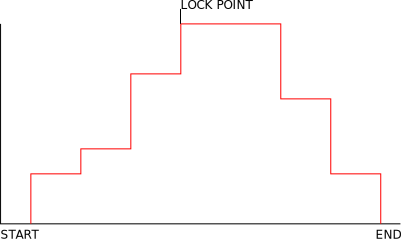
\includegraphics[width=0.6\textwidth]{out/two_phase_locking.eps}
  \caption{Two Phase Locking}
  \label{fig:two_phase_locking}
\end{figure}
\FloatBarrier

When releasing locks sequentially (as per figure \ref{fig:two_phase_locking}) it
is possible that a transaction $T_{1}$ may release the lock on an object $o_{1}$
which is then locked by transaction $T_{2}$.

If $T_{1}$ aborts before completion then $T_{2}$ will have read dirty data from
$o_{1}$ and will also need to abort (cascade abort).

This can be avoided using strict two phase locking where all the locks are
released simultaneously at the end of the transaction.

\begin{figure}[h!]
  \centering
  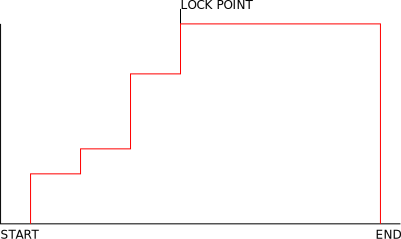
\includegraphics[width=0.6\textwidth]{out/strict_two_phase_locking.eps}
  \caption{Strict Two Phase Locking}
  \label{fig:strict_two_phase_locking}
\end{figure}
\FloatBarrier

Strict two phase locking ensured the consistency (C) and independence (I)
ACID properties.

\subsubsection{Deadlock Prevention}

Prevent wait for cycles caused by two transactions attempting to acquire locks
on objects held by the other transaction.

\Para{Simple approach}

\begin{itemize}
  \item Transactions never wait
  \item If lock on object is held by another transaction $T_{2}$ then $T_{1}$
        aborts
  \item Simple and easy to implement
  \item Effective if conflicts are rare
\end{itemize}

\Para{Timestamp Based}

Another approach is to permit waiting only if there is no danger of deadlock.

To do this transactions are assigned timestamps such that they are totally
ordered, these timestamps are then used in conflict resolution.

\begin{figure}[h]
  \centering
  \begin{subfigure}[b]{0.4\textwidth}
    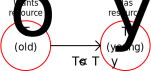
\includegraphics[width=0.8\textwidth]{out/deadlock_prevention_old-young.eps}
    \caption{Old - Young}
    \label{fig:deadlock_prevention_old-young}
  \end{subfigure}
  \begin{subfigure}[b]{0.4\textwidth}
    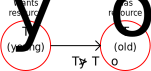
\includegraphics[width=0.8\textwidth]{out/deadlock_prevention_young-old.eps}
    \caption{Young - Old}
    \label{fig:deadlock_prevention_young-old}
  \end{subfigure}
  \caption{Deadlock prevention scenarios}
  \label{fig:deadlock_prevention}
\end{figure}
\FloatBarrier

\begin{description}
  \item[Wait-Die] \hfill \\
    \begin{itemize}
      \item Rule: If $T_{1} < T_{2}$ then $T_{1}$ waits, otherwise $T_{1}$
            aborts
      \item Old transactions (figure \ref{fig:deadlock_prevention_old-young})
            wait, newer transactions (figure
            \ref{fig:deadlock_prevention_young-old}) die
    \end{itemize}

  \item[Wound-Wait] \hfill \\
    \begin{itemize}
      \item Rule: If $T_{1} < T_{2}$ then $T_{1}$ forces $T_{2}$ to abort,
            otherwise $T_{1}$ waits
      \item Old transactions (figure \ref{fig:deadlock_prevention_old-young})
            abort/wound younger transactions, newer transactions (figure
            \ref{fig:deadlock_prevention_young-old}) wait
    \end{itemize}

\end{description}

\subsection{Commit Protocol}

The commit protocol ensures the atomicity (A) and durability (D) ACID
properties.

\begin{itemize}
  \item Changes to objects are made on copies of the object
  \item If transaction is aborted these copies are discarded
  \item If transaction is committed then changes are saved back to non-volatile
        storage
  \item This required a multi-pass commit protocol as changes must be made on
        either every node or no nodes
\end{itemize}

\subsubsection{Two Phase Commit}

\begin{itemize}
  \item Termination of the transaction is carried out by the client
        (coordinator).
  \item The first phase determines the outcome of the transaction
  \item The second phase is used to enforce the outcome
  \item Every node maintains a transaction log:
    \begin{itemize}
      \item Maintains information about transactions the node is taking part in
      \item Writing to log file is ensured to be atomic
      \item Stored on non-volatile storage
    \end{itemize}
  \item Every node has a recovery manager that executes when the node recovers
        from a crash
    \begin{itemize}
      \item Scans transaction log and determines actions required
      \item Tries to terminate all transactions that were active at the time of
            crash
    \end{itemize}
\end{itemize}

\Para{Phase 1}

\begin{minipage}[t]{0.5\textwidth}
  Coordinator

  \begin{enumerate}
    \item[1] Send \textit{get ready} message to all servers
    \item[2] Wait with timeout for reply from all servers
    \item[3] If all servers replay with \texttt{yes} then verdict is commit, if
             any one server replies with \textit{no} then verdict is abort
    \item[4] If verdict is commit then write transaction ID and server node
             addresses to the transaction log
  \end{enumerate}
\end{minipage}%
\begin{minipage}[t]{0.5\textwidth}
  Server

  \begin{enumerate}
    \item[1]   Wait with timeout fro \textit{get ready} command from coordinator
    \item[2]   If timeout elapses then abort transaction
    \item[3.1] If server does not want to commit then reply \textit{no}
    \item[3.2] Otherwise write transaction ID and coordinator node address to
               the transaction log and reply \textit{yes}
  \end{enumerate}
\end{minipage}

\Para{Phase 2}

\begin{minipage}[t]{0.5\textwidth}
  Coordinator

  \begin{enumerate}
    \item[1] Send verdict to all servers
  \end{enumerate}
\end{minipage}%
\begin{minipage}[t]{0.5\textwidth}
  Server

  \begin{enumerate}
    \item[1]   Wait without timeout for verdict from coordinator
    \item[2.1] If verdict is commit then store the copies of the objects on the
               stable data store
    \item[2.2] Otherwise if verdict is abort then discard the copies
  \end{enumerate}
\end{minipage}

\Para{Remarks}

\begin{itemize}
  \item In phase 1 any server can replay \textit{no}, this acts as a veto for
        the entire transaction, only one server needs to reply \texttt{no} for
        the transaction to be aborted
  \item In phase 1 if a server replies \textit{yes} then it is in a position
        to either commit or abort as it holds both original and modified
        versions of the objects
  \item Once a server replies \textit{yes} it must wait for the verdict from
        the coordinator
  \item If information about a transaction is missing in a transaction log then
        the transaction will eventually abort (this can happen if a node crashes
        just before the log is written)
  \item If a server crashes after writing to the transaction log then the
        recovery manager reads this log to decide (after communication with the
        coordinator) if it should commit or abort
  \item This protocol is a blocking protocol
  \item If the coordinator crashes in phase 2 and is not restarted then some
        servers may wait indefinitely
\end{itemize}

\subsection{Lock Free Transactions}

TODO

\end{document}
